%!TEX root = presentazionelancia.tex
\section{Consistency \& Failures}
\begin{frame}[t]\frametitle{Consistency}
	Under normal operation, TAO is \emph{eventually consistent}

	Replication lag usually < 1"

	Race conditions are resolved by using version numbers

	In special ``\emph{critical}" situation a read can be forwarded to database to ensure to read from a consistent source of truth. (Useful for auth procedures)

\end{frame}

\begin{frame}[t]\frametitle{Detecting Failures}
    Each TAO server stores per-destination time-outs
    \begin{itemize}
    	\item if several time-outs occur, hosts are marked as down
    	\item subsequent requests are aborted
    	\item Tao reacts trying to route around failures (favouring availability over consistency)
    	\item Down hosts are actively probed to check if recover
    \end{itemize}
    \centering
    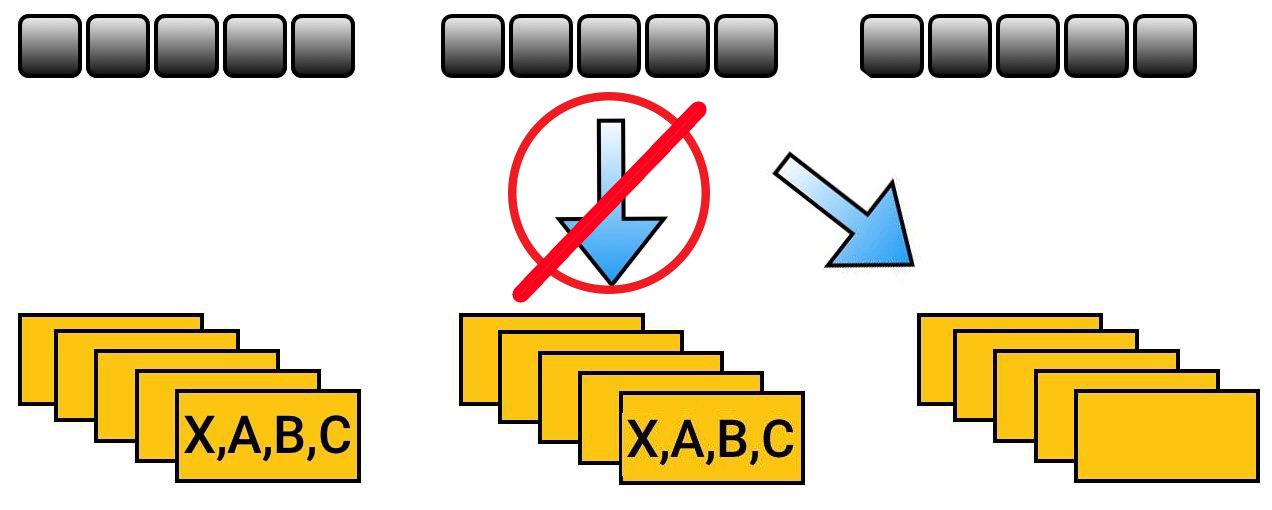
\includegraphics[width=0.6\textwidth]{figs/fail.jpg}

\end{frame}

\begin{frame}[c]\frametitle{Handling Failures}
    \begin{description}
    	\item[Database Fail] Db can crash or be off-line for maintenance. 
    	\begin{itemize}
    		\item If master db is down, a slave is promoted to new master
    		\item If a slave db is down, cache miss are redirected to TAO leaders in master region
    	\end{itemize}
    	\item[Leader Fail] Followers re-route requests around it
    	\begin{itemize}
    		\item Read miss goes directly to db
    		\item Write are routed to a random member of the leader tier
    	\end{itemize}
    \end{description}
\end{frame}

\begin{frame}[c]\frametitle{Handling Failures (2)}
    \begin{description}
    	\item[Invalidation Fail] Leader can't contact a follower during a cache invalidation message
    	\begin{itemize}
    		\item Leader queues message 
    		\item If Leader also crash message are lost so new leader send bulk invalidation
    	\end{itemize}
    	\item[Follower Fail] Followers in others tiers share the responsibility of it's shard
    	\begin{itemize}
    		\item Tao client have a primary tier and a backup tier
    	\end{itemize}
    \end{description}


\end{frame}
